\documentclass[conference]{IEEEtran}
\usepackage[affil-it]{authblk}
\IEEEoverridecommandlockouts
% The preceding line is only needed to identify funding in the first footnote. If that is unneeded, please comment it out.
\usepackage{cite}
\usepackage{amsmath,amssymb,amsfonts}
\usepackage{algorithmic}
\usepackage{graphicx}
\usepackage{textcomp}
\usepackage{xcolor}
\usepackage{fancyhdr} % Added for footer
\pagestyle{fancy}
\fancyhf{}
\fancyfoot[C]{ISBN: 979-8-3503-9838-0}
\fancyfoot[R]{Page \thepage\ of 4}
\renewcommand{\headrulewidth}{0pt}
\def\BibTeX{{\rm B\kern-.05em{\sc i\kern-.025em b}\kern-.08em
    T\kern-.1667em\lower.7ex\hbox{E}\kern-.125emX}}
\begin{document}

\title{\fontsize{16}{24}\bfseries\selectfont A High Performance Computing Platform for Big Biological Data Analysis}

\author{Chang-Wei Yeh, Chieh-Wei Huang, Chia-Lee Yang*, Yu-Tai Wang}

\renewcommand\Affilfont{\fontsize{10}{13}\selectfont}
\affil{\normalfont National Centre for High-Performance Computing,\\
\normalfont National Applied Research Laboratories, Hsinchu, Taiwan\\
\normalfont Corresponding author: Chia-Lee Yang, TEL: 886-35776085, E-mail: joy.yang@nchc.org.tw}

\maketitle
\thispagestyle{fancy}

\begin{abstract}
With the rapid progress of high-throughput sequencing projects, biological data is growing exponentially, creating a need for efficient and scalable algorithms and high-performance computing (HPC) platforms for big biological data analysis. However, traditional HPC platforms are inadequate for meeting the demand for rapid data analysis tasks in bioinformatics research. Analyzing biological sequence data is challenging due to its complexity and long computing time. This poses challenges for researchers to gain a deep understanding of biological functions. Thus, this research presents a large-scale biological data analysis platform enabled by an HPC infrastructure for genomic sequencing data and protein structure analysis. A practical case of HPC platforms for big biological data analytics in Taiwan is also presented. By using a reconfigurable HPC platform, the computational bottleneck can be removed, and data analysis can be accelerated. The platform enables researchers to gain profound insights into the deepest biological functions by addressing the challenges of big biological data analysis.
\end{abstract}

\begin{IEEEkeywords}
High Performance Computing (HPC), Big Data, Genomic sequencing, Protein structure analysis, Biological Data Analysis
\end{IEEEkeywords}

\section*{\textbf{Introduction}}
High Performance Computing (HPC) has increasingly been utilized in the field of biology, especially during the Covid-19 pandemic. Researchers have used HPC for drug discovery, variant modeling, and analyzing antibody-virus interactions \cite{b1}. Despite the growing importance of HPC, biological analysis remains a challenging application due to its unstructured data format and complex access patterns for analyzing colossal amounts of genomic data \cite{b2}. While traditional general-purpose HPC architectures are optimized for fast processing of parallel data and executing complex computations, the specialized computing requirements of biology have led to the rapid evolution of HPC systems, with new architecture constantly being developed and optimized for sophisticated data usage.

One particularly significant application is the widely-used biological sequence analysis, which has become essential for basic genomic and molecular biology research and has a major impact on biomedicine. Genomic sequencing data and protein structure analysis are critical for this application and have been specialized for speed at the expense of general applicability. With the exponential growth of biological databases resulting from the human genome project (HGP), supercomputers and other parallel architectures such as special purpose Very Large Scale Integration (VLSI) chips, Graphics Processing Units (GPUs), and Field Programmable Gate Arrays (FPGAs) have gained popularity as acceleration platforms. However, choosing an acceleration platform always involves trade-offs between factors such as area, speed, power consumption, cost, development time, and reusability \cite{b3}. To leverage the low-cost advantages of shared facilities and the computational efficiency of specialized chips, this paper presents a large-scale biological data analysis platform enabled by an HPC infrastructure for genomic sequencing data and protein structure analysis. A practical case of HPC platforms for big biological data analytics in Taiwan is also presented in this paper.

\section*{\textbf{Computational Performance Comparison}}
To compare the performance of different computational architectures in biological data processing, we analyze execution times for key bioinformatics tasks:

\begin{table}[h]
    \centering
    \resizebox{\columnwidth}{!}{
        \begin{tabular}{|c|c|c|c|}
            \hline
            \textbf{Platform} & \textbf{Genome Assembly (min)} & \textbf{Protein Folding (hrs)} & \textbf{Data Transfer (GB/s)} \\
            \hline
            CPU Cluster & 120 & 10 & 1.5 \\
            GPU Cluster & 45 & 3 & 5.0 \\
            FPGA System & 30 & 2 & 4.5 \\
            \hline
        \end{tabular}
    }
    \vspace{5pt}
    \caption{Performance comparison of different HPC architectures.}
    \label{tab:performance}
\end{table}

\section*{\textbf{Mathematical Model for Parallel Computing}}
The speedup achieved in parallel computing can be estimated using Amdahl’s Law:

\begin{equation}
    S = \frac{1}{(1 - P) + \frac{P}{N}}
\end{equation}

where:
\begin{itemize}
    \item $S$ is the speedup factor,
    \item $P$ is the parallelizable portion of the task,
    \item $N$ is the number of processing units.
\end{itemize}

This equation helps evaluate the benefits of increasing parallelization in HPC bioinformatics workloads.

Another important model in HPC is Gustafson’s Law, which considers scalability:

\begin{equation}
    S = N - (1 - P)N
\end{equation}

This equation shows that as the number of processors increases, the speedup is less constrained by the non-parallelizable portion of the workload.

\section*{\textbf{Related Work}}
The growth of computational power has brought about a revolution in the field of biology, leading to its recognition as an informational science \cite{b4}. Bioinformatics has become an indispensable tool for biological research, with omics fields like genomics, proteomics, and metabolomics now considered to be big data sciences \cite{b5}. Biological sequence analysis is a widely used bioinformatics application that is critical for basic research and several areas of biomedicine, including knowledge-based drug design, forensic DNA analysis, and agricultural biotechnology. Various techniques such as sequence alignment, sequence database searching, motif and pattern discovery, reconstruction of evolutionary relationships, genome assembly, and comparison are involved in the analysis of biological sequences.

One of the most significant challenges in biological sequence analysis is the computational complexity of processing vast amounts of genomic data. To overcome this challenge, researchers have turned to HPC infrastructures that offer distributed computing and data resources such as processing, network bandwidth, and storage. Biological sequence analysis is currently one of the most computationally demanding tasks for most supercomputing centers, requiring high levels of compute load, communication speed, and memory load. Thus, some supercomputing centers develop new architectures for biological sequence analysis. For example, The Pittsburgh Supercomputing Center has developed Bridges 2015 \cite{b6}. Pittsburgh Supercomputing Center's Bridges is a user-focused research system that integrates advanced memory technologies. It features three tiers of processing nodes, persistent databases, and web nodes, and supports research communities through interactivity, gateways, tools, and virtualization. Bridges also ensures optimal data handling with state-of-the-art CPUs and GPUs and multiple filesystems, while promoting data-intensive science awareness through interoperability with other cyberinfrastructure resources.

In 2016, the Italian supercomputing center launched ELIXIR-IT HPC@CINECA, which provides streamlined access to HPC resources for bioinformatics \cite{b7}. Resources can be accessed through web front-ends to dedicated workflows developed at CINECA or through a standard command-line interface tailored for bioinformatics data analysis, allowing the biomedical research community to utilize a production-scale environment continuously updated with the latest publicly available reference datasets and bioinformatics tools.

\section*{\textbf{Solutions}}
The National Center for High-Performance Computing (NCHC) is the exclusive national-level supercomputing center in Taiwan, serving as a vital component of the country's information infrastructure. NCHC’s primary objective is to provide general-purpose HPC resources for a wide range of fundamental research endeavors. To enable biological researchers in Taiwan to overcome the obstacles associated with using HPC, the NCHC has developed the "NCHC Biological Core Facility (NBCF)," which is part of a long-term national project called the "National Core Facility for Biopharmaceuticals."

NBCF provides exclusive supercomputing and storage capacity, biological proprietary computing nodes, public domain analysis workflows and software, user-friendly interfaces, commercial software and hardware for genome analysis, and access to essential technology consultation, education, and training. User payments are required to prevent unnecessary resource wastage.

\subsection{Containerized Workflow Services}
Galaxy \cite{b8} is a web-based analysis platform for life science research that provides biological researchers to manage and run bioinformatics tools and workflows on HPC systems. However, despite its advantages, there are significant constraints for researchers. The Galaxy is designed as a centralized site, which means that researchers cannot personalize their own versions of Galaxy. Moreover, at most supercomputing centers, HPC services are usually restricted to computing nodes, and running personal Galaxy services on a login node is prohibited due to security policies. Additionally, Galaxy employs a single administrative account to submit jobs, making it challenging to attribute usage fees to different users.

To address these challenges, NBCF has introduced DJXpert, a web-based platform for HPC. DJXpert submits a slurm queue job to activate Singularity/Docker service and uses ssh forwarding schedule to provide a connection between the user and HPC via DJXpert. This allows users to run their Galaxy services on computing nodes through their own accounts, making it easier for the system to attribute usage fees. The Galaxy container has also been modified to use HPC’s job scheduler (SLURM), enabling Galaxy to submit jobs to other computing nodes and scale up the system. Additionally, during service initialization, the database and main program are separated to ensure that users have their previously-built sites after reboot. This service model can be extended to other interactive tools such as R studio and Jupyter notebook, making HPC-based core services more user-friendly.

\begin{figure}[htbp]
    \centering
    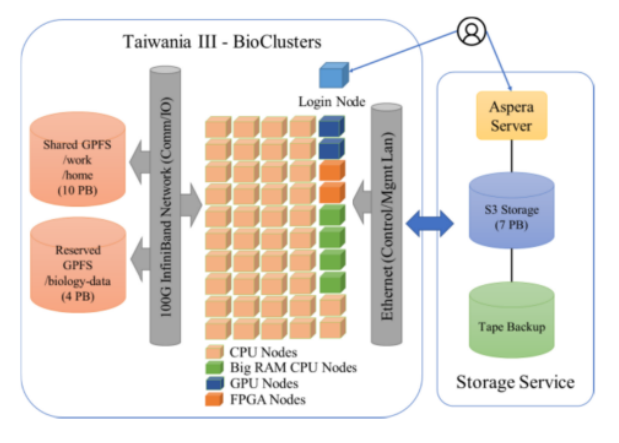
\includegraphics[width=\linewidth]{fig1.png} % Replace with the actual filename
    \caption{NBCF cluster and storage service}
    \label{fig1}
\end{figure}

\subsection{Heterogeneous Computing Nodes}
Traditionally, most Next Generation Sequencing (NGS) tools run on CPUs, while GPUs are mostly used for predicting protein structure. However, as genomics data grows in size, the analysis process becomes increasingly time-consuming. To address this, FPGA and GPU technologies have been used to accelerate gene analysis processes, particularly for memory-intensive tasks such as De-novo Assembly of unknown mammal or plant genomes \cite{b9}.

To support this need for heterogeneous computing, NBCF provides a range of computing nodes with varying capabilities. As of 2021, NBCF offers a total of 51 computing nodes, including 39 nodes with 56 cores and 192 GB of memory, 6 nodes with 384 GB of memory, 4 nodes with ultra-large memory in the TB range, and two nodes equipped with 8 NVIDIA V100 GPUs. Additionally, the NCHC offers FPGA-accelerated gene analysis services through the Illumina DRAGEN platform.

\subsection{Data Loading Optimization}
To transfer large amounts of data to an HPC system, ample storage space and high network speeds are necessary. To minimize the need for data migration, maintaining a copy of commonly used data on the HPC's storage is also essential. To handle the vast amount of biological analysis data, NBCF provides users with high-speed parallel file systems and object-based storage space for data backup. These resources include a personal high-speed calculation space of 100 GB in the home directory, a personal dedicated work area storage space of 1.5 TB, and up to 4 PB of shared space for file sharing (Fig 1).

Additionally, data storage can be customized to meet the specific needs of laboratories, including file sharing. To ensure fast and efficient data transmission, NBCF offers a high-speed file transfer mechanism that utilizes a dedicated server and IBM Aspera high-speed transmission software with a bandwidth of 1G, minimizing data transfer time. NBCF also provides common reference sequences and annotation data onto the HPC for universal access by all users. The research project data, which is hosted on the HPC's storage, can be transferred to users' working space upon approval, further reducing the need for data migration.

\subsection{Scheduling design based on memory size}
Traditional HPC scheduling is typically based on the number of cores available in a given system. The scheduler allocates jobs to available cores, and when all cores are occupied, jobs are queued until resources become available. This method works well for many types of applications, but for biological analysis, where memory requirements can vary widely, it may result in inefficient resource utilization and long queue times. Biological applications often require a large amount of memory, which can result in long queuing times when core count is used as the basis for scheduling in supercomputing centers.

By using memory size as the basis for scheduling, the queuing times can be reduced and the computational efficiency can be improved for these memory-intensive applications \cite{b10}. While this method represents a significant breakthrough in scaling, the memory overhead for this particular implementation is prohibitive, in the sense that simulations of RNA complexes.

\begin{figure}[htbp]
    \centering
    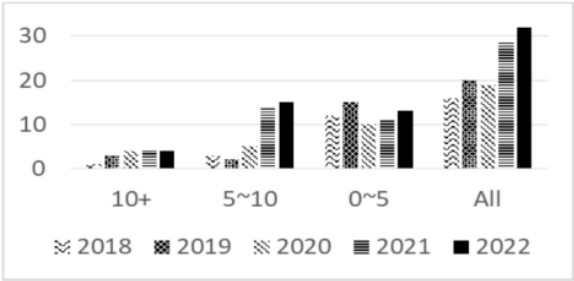
\includegraphics[width=\linewidth]{fig2.png} % Replace with actual filename
    \caption{Number of Published Papers Acknowledging NBCF Support.}
    \label{fig2}
\end{figure}

\section*{\textbf{Results}}
The NBCF was developed to support biological research by providing exclusive supercomputing and storage capacity, user-friendly interfaces, commercial software and hardware for genome analysis, and access to essential technology consultation, education, and training. The NBCF introduces three novelties: containerized workflow services, heterogeneous computing nodes, and data loading optimization. In addition, the NBCF uses a scheduling design based on memory size to reduce queuing times and improve computational efficiency for memory-intensive biological applications.

Every year, the NBCF provides services to about 30 academic and research institutions, as well as 200 to 300 biological researchers in Taiwan who apply to use the genome and protein analysis platform services. The NCHC's contributions have been widely recognized, with more than 100 international journal publications acknowledging NBCF in their acknowledgments. One of these publications even had an impact factor greater than 66 (Fig. 2).

\begin{thebibliography}{00}
\bibitem{b1} J. J. Hack and M. E. Papka, “The US high-performance computing consortium in the fight against COVID-19,” Computing in Science \& Engineering, vol. 22, no. 6, pp. 75-80, 2020.
\bibitem{b2} S. Pal, S. Mondal, G. Das et al., “Big data in biology: The hope and present-day challenges in it,” Gene Reports, vol. 21, pp. 100869, 2020.
\bibitem{b3} M. N.M. Isa, “High performance reconfigurable architectures for biological sequence alignment,” 2013.
\bibitem{b4} Z. Yin, H. Lan, G. Tan et al., “Computing platforms for big biological data analytics: perspectives and challenges,” Computational and Structural Biotechnology Journal, vol. 15, pp. 403-411, 2017.
\bibitem{b5} G. Dall’Alba, P. L. Casa, F. P. d. Abreu et al., “A Survey of Biological Data in a Big Data Perspective,” Big Data, vol. 10, no. 4, pp. 279-297, 2022.
\bibitem{b6} N. A. Nystrom, M. J. Levine, R. Z. Roskies et al., “Bridges: a uniquely flexible HPC resource for new communities and data analytics.”
\bibitem{b7} T. Castrignano, S. Gioiosa, T. Flati et al., “ELIXIR-IT HPC@ CINECA: high performance computing resources for the bioinformatics community,” BMC bioinformatics, vol. 21, pp. 1-17, 2020.
\bibitem{b8} D. Blankenberg, G. V. Kuster, N. Coraor et al., “Galaxy: a web-based genome analysis tool for experimentalists,” Current protocols in molecular biology, vol. 89, no. 1, pp. 19.10.1-19.10.21, 2010.
\bibitem{b9} L. Guo, J. Lau, Z. Ruan et al., “Hardware acceleration of long read pairwise overlapping in genome sequencing: A race between FPGA and GPU.”
\bibitem{b10} S. Coakley, M. Gheorghe, M. Holcombe et al., “Exploitation of high performance computing in the FLAME agent-based simulation framework.”
\end{thebibliography}

\end{document}